\documentclass[a4paper,12pt]{article}
\usepackage[utf8]{inputenc}
\usepackage[top=2cm,bottom=2.54cm,left=2.54cm,right=2.54cm]{geometry}
\usepackage[namelimits]{amsmath} 
\usepackage{amssymb}             
\usepackage{amsfonts}            
\usepackage{mathrsfs}            
\usepackage{graphicx}
\usepackage{subfigure}
\usepackage{multirow}
\usepackage{listings}
\usepackage{diagbox}
\usepackage{slashbox}
\lstset{language=Matlab}
\lstset{breaklines}
\lstset{extendedchars=false}

\title{Fintech545 Homework 4}
\author{qw112 Qiyu Wu}
\date{}

\begin{document}
\maketitle
\subsection*{Question 1. Normal and a Generalized T Distribution}
For the problem, I use MLE to fit a normal Distribution and a generalized t distribution.
\begin{center}
    \begin{tabular}{ |c|c|c|}
     \hline
       & VaR & ES\\
     \hline
     Normal Distribution&0.0822&0.1022\\
     T Distribution&0.0763&0.1142\\
     \hline
    \end{tabular}
\end{center}
\begin{center}
    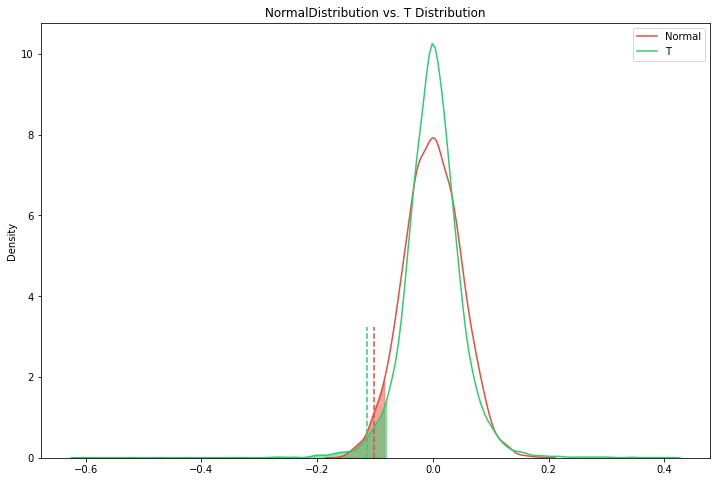
\includegraphics[width=10cm]{output.png}
\end{center}
\begin{itemize}
    \item \textbf{Expected Shortfall: } From the above graph, we can see that the T distribution has a fat tail, which contributes the increase of Expected shortfall. This is because Expected shortfall is the expectation over the whole left tail area.
    \item \textbf{VaR: } From the table, we can find that T distribution has a lower VaR value. It is because the T distribution has a lower sigma than normal distribution here, which lead that the distances of these two distributions are different.
\end{itemize}

\subsection*{Question 2. Library: QuantRisk}
I have create a library for my previous functions used in the homework. All the functions have been tested by using test suite. For files named mill and ts\_sim, they has been proved based on the previous homework.

\newpage
\subsection*{Question 3. Portfolio Fitting with T Distribution}

\begin{center}
    \begin{tabular}{ c|c|c|c|c}
     \hline
      VaR(\$) & Portfolio A & Portfolio B & Portfolio C & Total\\
     \hline
     Normal VaR&5618.944064&4382.329498&3754.823054	&13486.8134\\
     T VaR &7321.87367&6083.282769&4213.866454&17316.648493\\
     T ES &9697.83096&8192.52733&5858.4264&23507.5362\\
     \hline
    \end{tabular}
\end{center}

\begin{itemize}
    \item From the above table, we can find that Normal VaR has the lowest estimation about risk. It is because that normal distribution has the more narrow tail than t distribution;
    \item When compared to Expected Shortfall, VaR generally is smaller than it. It is because of the fat tail of T distribution, which contributes to the higher estimation of risk level.
\end{itemize}

\end{document}